\section{How to contribute}

The specifications of a given data level format defines the names and semantics of data and header fields. Such specifications are made easy to understand. Specifications of this format are currently written that can form the basis for prototyping for data producers (mainly existing IACTs and simulated CTA data) and consumers (mainly science tool codes). We include example files and some explanations, in addition to the detailed specifications for a given format. 

The scope is high-level data, starting with event lists and instrument response functions (IRFs), what is called "data level 3" (DL3) in CTA. The first stable release (archived on Zenodo with a DOI) is coming soon.

If you want to contribute, it is simple:

\begin{itemize}
\item{}Use the existing format and give feedbacks. Propose additions and changes.
\item{}Join the mailing list (see next section). Send an e-mail with an idea or proposal.
\item{}Create a Github account. File an issue with a correction or make a pull request proposing additions.
\end{itemize}

No formal approval process is in place yet as this is a very recent effort.

\subsection{Resources}

\begin{itemize}
\item{} Mailing list for announcements and high level discussions (75 members, including people from all major gamma-ray collaborations :\\     \url{https://lists.nasa.gov/mailman/listinfo/open-gamma-ray-astro}
\item{}Github issues and pull requests are used for detailed discussions:\\ \url{https://github.com/open-gamma-ray-astro/gamma-astro-data-formats}
\item{}Data format specifications in HTML and PDF format, including example files:\\ \url{https://gamma-astro-data-formats.readthedocs.io/}
\end{itemize}

The specs are written in a markup format called "restructured text" (RST),
which gets transformed by Sphinx to HTML or PDF, the latest rendered version is always available online (see Figure~\ref{fig:webpage}).

\begin{figure}[tb]
\centerline{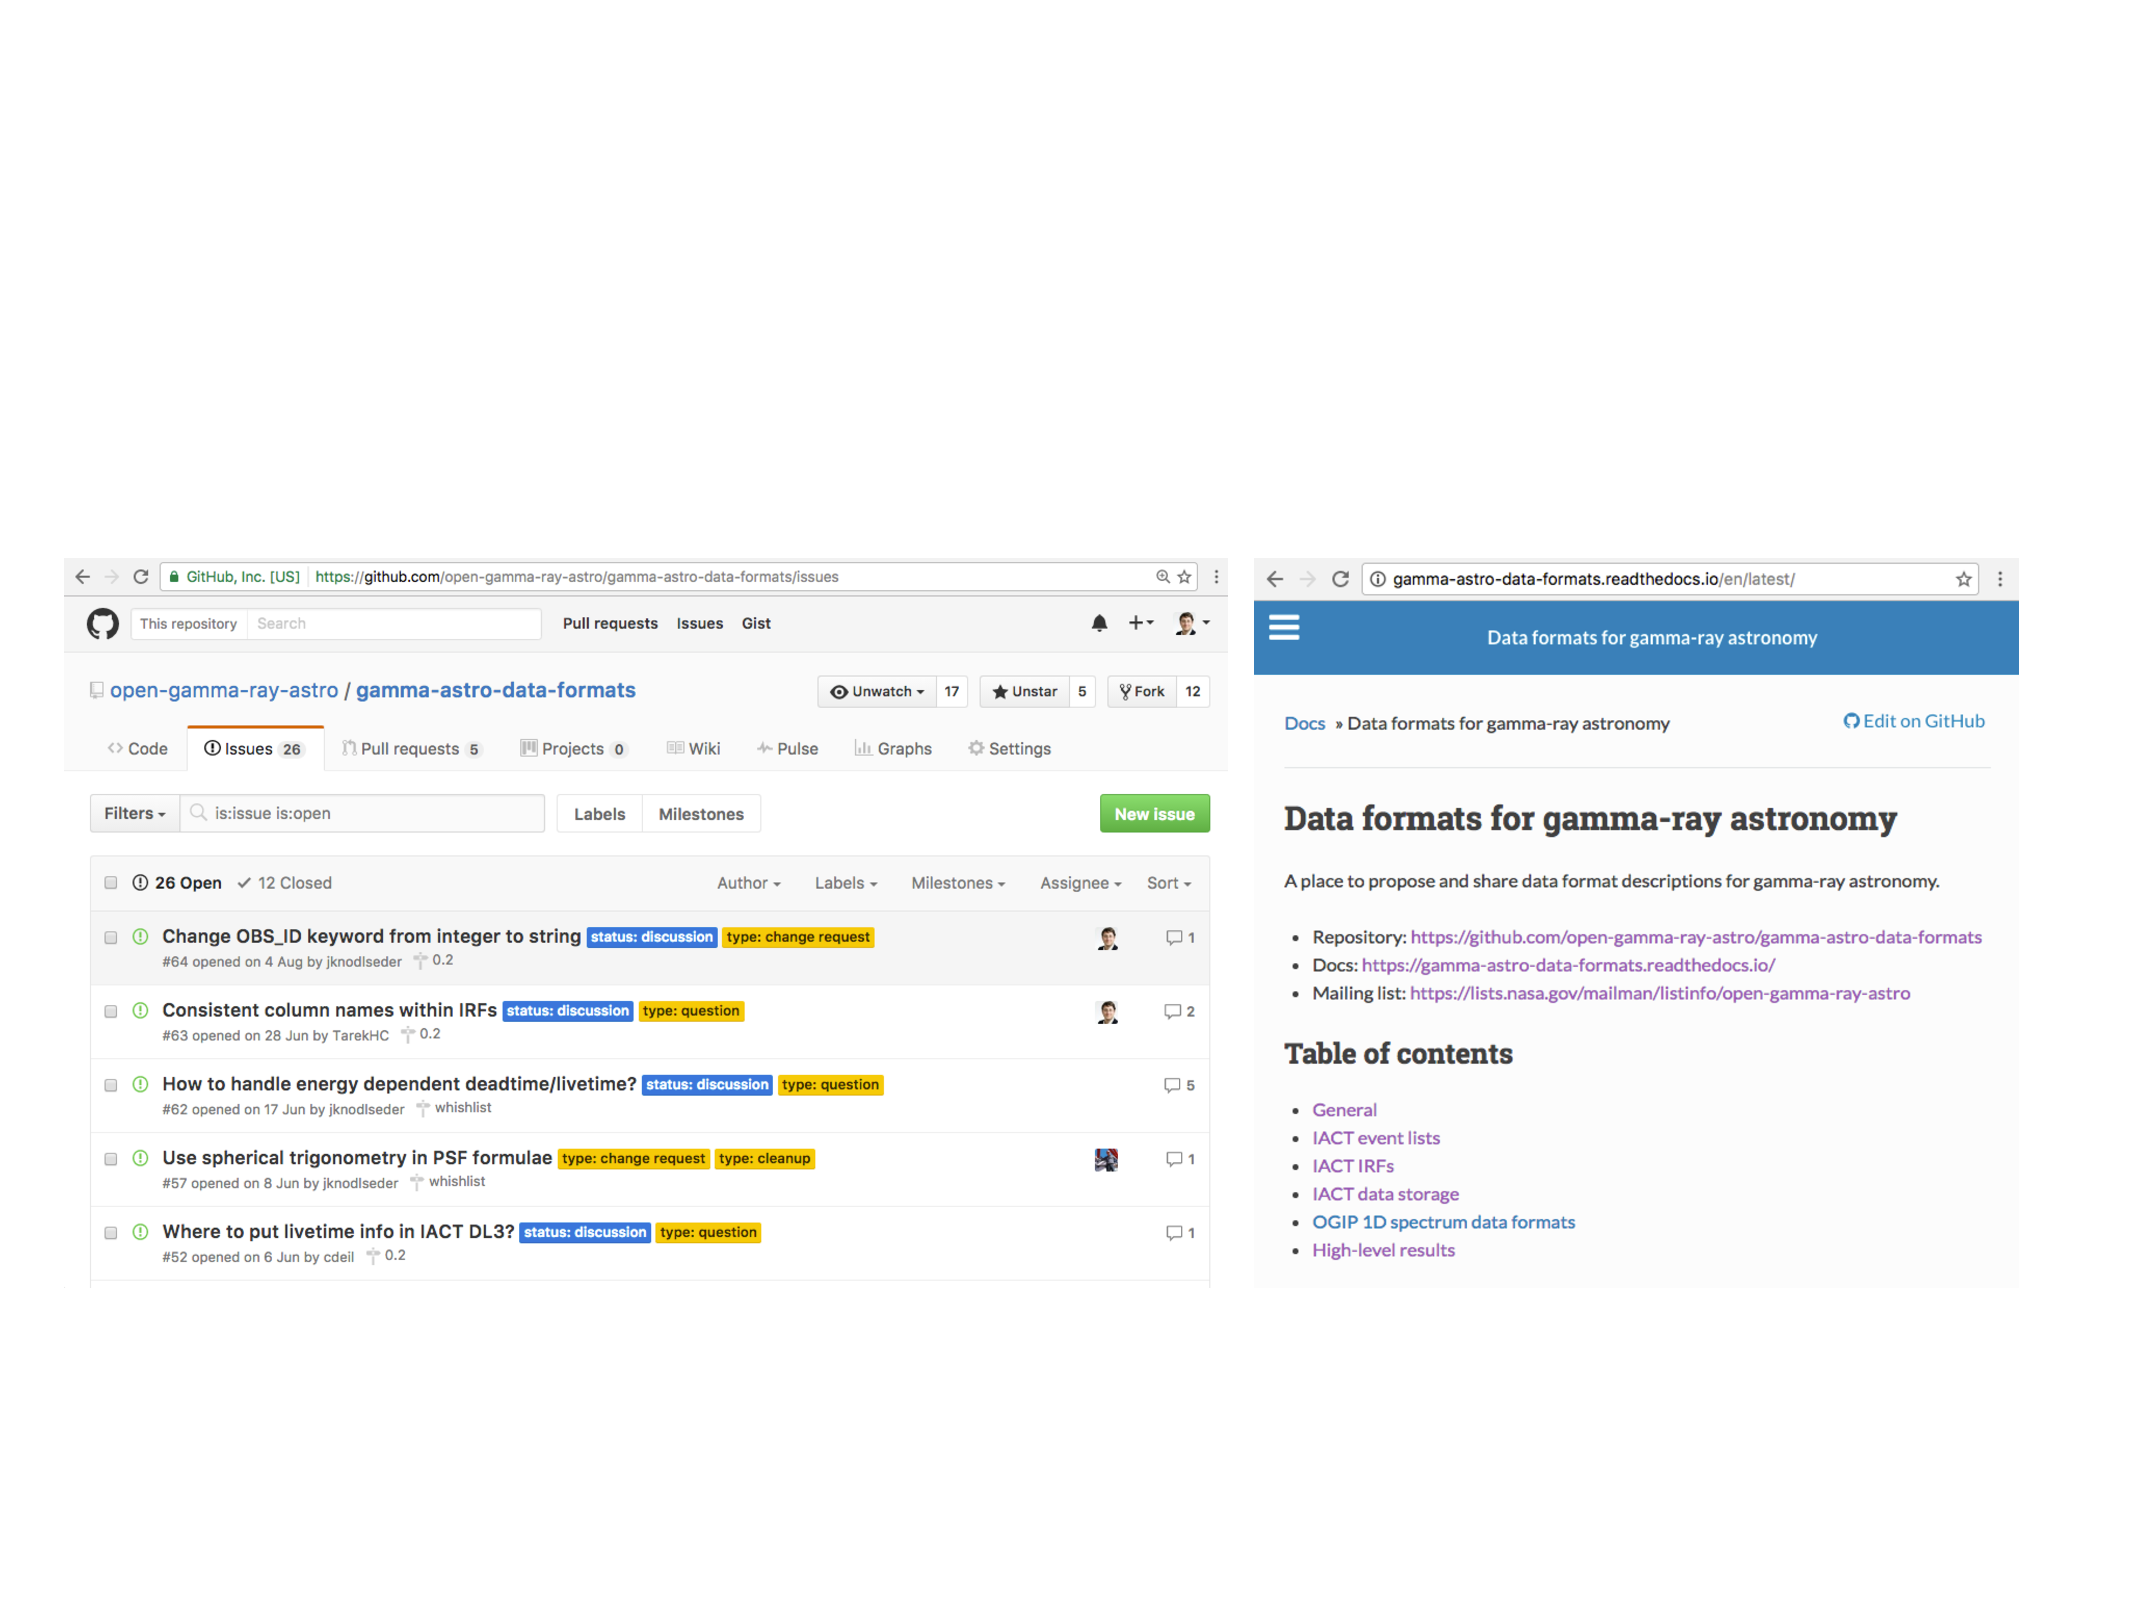
\includegraphics[width=\textwidth]{figures/webpage}}
\caption{
\emph{Left:} \texttt{gamma-astro-data-formats} Github issue tracker with ongoing discussions. \emph{Right:} latest version of the \texttt{gamma-astro-data-formats} specifications on Read the Docs (PDF and older tagged versions also available).
}
\label{fig:webpage}
\end{figure}
